\section{Einleitung Agile Softwareentwicklung}
- ABHOLUNG\\
Vorschlag: Im Laufe der Vorlesung wurden immer wieder IT-gestützte Ingenieurwerkzeuge und deren Einsatz im Produktentstehungsprozess erwähnt. \cite{Daberkow2022} Aber wie ist eigentlich das Vorgehen, wenn das IT-Tool nicht bei beispielsweise beim Anforderungsmanagement oder der Entwicklung in der Konstruktion unterstützen soll, sondern Software selbst entwickelt werden soll? --> Wollen wir im Verlauf der Präsentation am Beispiel Automotive Bereich erläutern. \\
- Kernaussage\\
Vorschlag: Was bedeutet eigentlich agil sein? Agil sein bedeutet, dass man schnell und wendig ist. Das ist auch das Ziel der agilen Softwareentwicklung. Es soll mit ständig angepasstem Vorgehen schnell vorzeigbare Ergebnisse erreicht werden. \cite{wolf2011agile}\\
- Was ist agile SW-Entw.\\
- Was erhofft man sich vom Einsatz agiler Entwicklungsmethoden (siehe Kernaussage?)\\
\glqq Agile Softwareentwicklung ist ein Sammelbegriff für eine Reihe von Frameworks und Praktiken, die auf den Werten und Grundsätzen beruhen, die im Manifest für agile Softwareentwicklung und den dahinter stehenden zwölf Prinzipien zum Ausdruck kommen.\grqq  \cite{agile101} Im Verlauf der Präsentation sollen diese Praktiken und Prinzipien in den Produktentstehungsprozess eingeordnet werden. \\
- Wieso wird agile Softwareentwicklung heute eingesetzt? + evtl. kurzer Vergleich zu V-Modell (sehe Vergleich eher hier: \ref{vergleich})\\ 

\section{Einordnung in den Produktentstehungsprozess}
- Eigene Prozessabläufe wurde gebildet, die sich nur mit Softwareentwicklung befassen\\
- Einordnen in Bild 2.9 + evtl. neuer Balken\\
- Embedded-Softwareentwicklung teilweise mit "Entwicklung Konstruktion E/E"-Balken verbunden\\
- Restliche Softwareentwicklung eher eigner Balken\\

\section{Agiler Prozessablauf an einem Beispiel im Automotive Bereich}
- Beispiel des SAFe Scaled Agile Framework\\ 
- Wie wird agile Softwareentwicklung im Unternehmen umgesetzt? \\
- z.b. Wie laufen die Prozesse SAFe ab, Wann ist wer beteiligt (Buisness owner -> product owner -> entwickler)\\
- Methoden wie Scrum, Ticketsystemen (Umsetzung), DevOps etc. \\ 
- Hier wird beschrieben wie sich Umternehmen bzw. Unternehmensbereich strukturiert (Abläufe/Prozesse/Schnittstellen/Personengruppen und ihre Aufgaben/Schnittstellen) \\ 
 
\section{Agile Methoden im Vergleich zum herkömmlichen Produktentstehungsprozess}\label{vergleich}

\begin{enumerate}
	\item Agile Manifesto Kernthese (1) besagt bereits dass Prozesse und Werkzeuge vernachlässigt werden sollen
	\item Auch (3) widerspricht langwierigen Genehmigungsprozessen zur Erstellung verbindlicher Dokumente für Anforderungsspezifikationen wie in einem Lasten-/Pflichtenheft
	\item Statt langwieriger \glqq systematische Erfassung, Analyse, 
	Prüfung, Aufbereitung, Dokumentation und Verfolgung von Anforderungen an ein Produkt\grqq{} \cite{Daberkow2022} sollen Anforderungen in einem iterativen Prozess in ständiger Kommunikation mit dem Kunden abgestimmt werden
\end{enumerate}

 \subsection{Agile gegenüber Lasten/Pflichtenheft}
 - Vergleich Agile / Lasten/Pflichtenheft Skript Kapitel 3.4 -> zum Beispiel auf Terminplanung und Komponentenbeschreibung eingehen\\


 

 \subsection{Besonderheiten der SW-Entwicklung für automobile Anwendungen}
 - ASPICE, höhere Sicherheitsanforderungen, Änderungen einpflegen, Testing Prozess (automatisiert, verschiedenen Ebenen, Von Unittest - bis Fahrzeugerprobung, sicherheitsrelevant)\\

\section{Fazit}
- RÜCKFÜHRUNG\\
- Zusammenfassung, Positionieren zur agilen Entwicklungsmethoden \\
- Ausblick: wird weiter entwicklet, recht neu, viele Unternehmen übernehmen zur Zeit agile Methoden/Strukture \\
- Erfordert Umstellung von Denkweisen/Mitarbeitern/Organisationen\\
\section{Ausblick}

\newpage
\listoffigures
\textbf{Einfügen Bilder nur zur automatischen abbildungsverzeichnis erstellung}
\begin{figure}[htb]
	\centering
	
\includegraphics[width=\textwidth]{img/agile_symbol.jpg}
	\caption[Symbolgraphik Agile (Quelle: stock.adobe.com)]{Symbolgraphik Agile (Quelle: stock.adobe.com)}
	\label{fig:agile}
\end{figure}

\begin{figure}[htb]
	\centering
	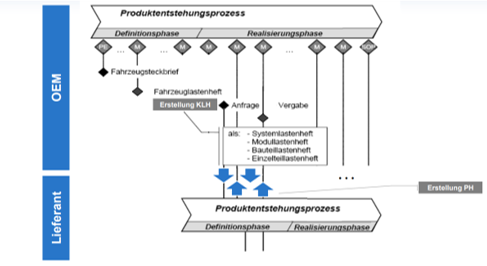
\includegraphics[width=\textwidth]{img/klh_produktentstehungsprozess.png}
	\caption[Komponentenlastenhefte im Produktentstehungsprozess (Quelle: \cite{Daberkow2022})]{Komponentenlastenhefte im Produktentstehungsprozess (Quelle: \cite{Daberkow2022})}
	\label{fig:klh}
\end{figure}

\begin{figure}[htb]
	\centering
	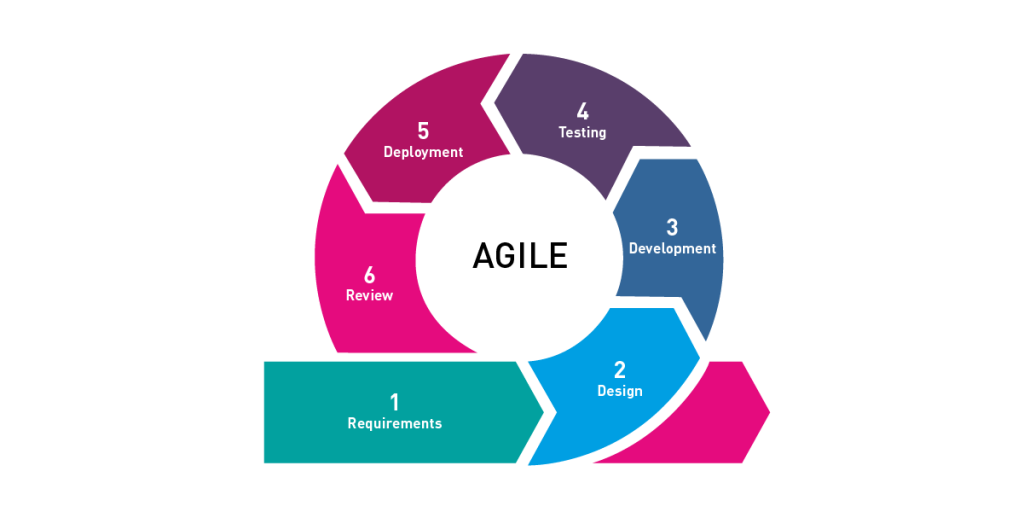
\includegraphics[width=\textwidth]{img/agile_cycle.png}
	\caption[Agiler Prozesszyklus Quelle: ]{Agiler Prozesszyklus}
	\label{fig:klh}
\end{figure}
